\documentclass[11pt]{article}
\usepackage[top=1.5cm,bottom=2cm,left=2cm,right= 2cm]{geometry}
\geometry{letterpaper}                   % ... or a4paper or a5paper or ... 
%\geometry{landscape}                % Activate for for rotated page geometry
\usepackage[parfill]{parskip}    % Activate to begin paragraphs with an empty line rather than an indent
\usepackage{graphicx}
\usepackage{amssymb}
\usepackage{epstopdf}
\usepackage{amsmath}            
\usepackage{multirow}    
\usepackage{multicol}    
\usepackage{changepage}
\usepackage{lscape}
\usepackage{enumitem}
\usepackage{ulem}
\DeclareGraphicsRule{.tif}{png}{.png}{`convert #1 `dirname #1`/`basename #1 .tif`.png}

\usepackage{xcolor}

\definecolor{oiB}{rgb}{.337,.608,.741}
\definecolor{oiR}{rgb}{.941,.318,.200}
\definecolor{oiG}{rgb}{.298,.447,.114}
\definecolor{oiY}{rgb}{.957,.863,0}

\definecolor{light}{rgb}{.337,.608,.741}
\definecolor{dark}{rgb}{.337,.608,.741}

\usepackage[colorlinks=false,pdfborder={0 0 0},urlcolor= dark,colorlinks=true,linkcolor=black]{hyperref}

\newcommand{\light}[1]{\textcolor{light}{\textbf{#1}}}
\newcommand{\dark}[1]{\textcolor{dark}{#1}}
\newcommand{\gray}[1]{\textcolor{gray}{#1}}


%\date{}                                           % Activate to display a given date or no date

\begin{document}

{\LARGE \textcolor{oiB}{Learning Objectives \hfill Chapter 8: Introduction to linear regression}} \\


%

\begin{enumerate}
\renewcommand\labelenumi{\textcolor{light}{\textbf{LO \theenumi.}}}

\item Define the explanatory variable as the independent variable (predictor), and the response variable as the dependent variable (predicted).

\item Plot the explanatory variable ($x$) on the x-axis and the response variable ($y$) on the y-axis, and fit a linear regression model
\[ y = \beta_0 + \beta_1 x,\]
where $\beta_0$ is the intercept, and $\beta_1$ is the slope.
\begin{itemize}
\item[-] Note that the point estimates (estimated from observed data) for $\beta_0$ and $\beta_1$ are $b_0$ and $b_1$, respectively.
\end{itemize}

\item When describing the association between two numerical variables, evaluate
\begin{itemize}
\item[-] direction: positive ($x \uparrow, y \uparrow$), negative ($x \downarrow, y \uparrow$)
\item[-] form: linear or not
\item[-] strength: determined by the scatter around the underlying relationship
\end{itemize}

\item Define correlation as the \emph{linear} association between two numerical variables.
\begin{itemize}
\item[-] Note that a relationship that is nonlinear is simply called an association.
\end{itemize}

\item Note that correlation coefficient ($r$, also called Pearson's $r$) the following properties:
\begin{enumerate}
\item[-] the magnitude (absolute value) of the correlation coefficient measures the strength of the linear association between two numerical variables
\item[-] the sign of the correlation coefficient indicates the direction of association
\item[-] the correlation coefficient is always between -1 and 1, inclusive, with -1 indicating perfect negative linear association, +1 indicating perfect positive linear association, and 0 indicating no \emph{linear} relationship
\item[-] the correlation coefficient is unitless
\item[-] since the correlation coefficient is unitless, it is not affected by changes in the center or scale of either variable (such as unit conversions)
\item[-] the correlation of X with Y is the same as of Y with X 
\item[-] the correlation coefficient is sensitive to outliers
\end{enumerate}

\item Recall that correlation does not imply causation.

\item Define residual ($e$) as the difference between the observed ($y$) and predicted ($\hat{y}$) values of the response variable.
\[ e_i = y_i - \hat{y}_i \]

\end{enumerate}

\gray{
{\it
\vspace{-0.55cm}
\begin{itemize}
\renewcommand{\labelitemi}{{\textcolor{dark}{$\ast$}}}
\item Reading: Section 8.1 of OpenIntro Statistics
\item Videos: 
\begin{itemize}
\item[-] Review: \href{http://www.youtube.com/watch?v=5zyruPbgxyM}{Correlation vs. causation}, YouTube (2:19)
\item[-] \href{http://www.youtube.com/watch?v=zPG4NjIkCjc}{Intro to Linear Regression}, YouTube (5:18) - very slow introduction to linear regression
\end{itemize}
\item Test yourself:
\begin{enumerate}
\item Someone hands you the scatter diagram shown below, but has forgotten to label the axes. Can you calculate the correlation coefficient? Or do you need the labels?
\begin{center}
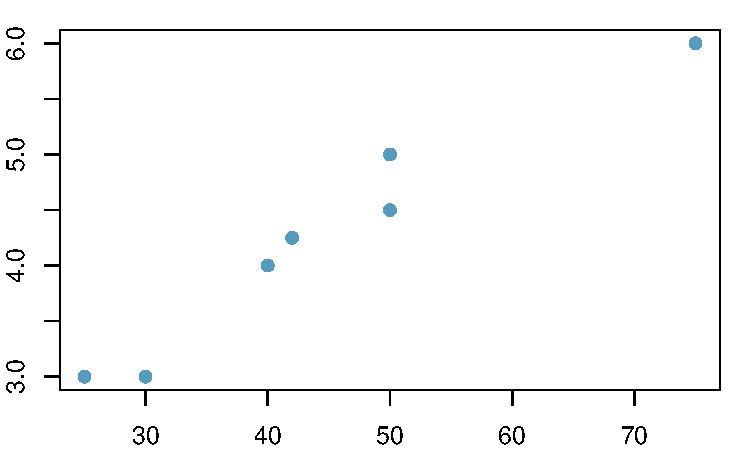
\includegraphics[width=0.4\textwidth]{figures/no_labels}
\end{center}
\item A teaching assistant gives a quiz. There are 10 questions on the quiz and no partial credit is given. After grading the papers the TA writes down for each student the number of questions the student got right and the number wrong. What is the correlation of the number of questions right and wrong? \\
Hint: Make up some data for number of questions right, calculate number of questions wrong, and plot them against each other.
\item Suppose you fit a linear regression model predicting score on an exam from number of hours studied. Say you've studied for 4 hours. Would you prefer to be on the line, below the line, or above the line? What would the residual for your score be (0, negative, or positive)?
\end{enumerate}
\end{itemize}
}}

%

\vspace{0.48cm}

%
\begin{enumerate}[resume]
\renewcommand\labelenumi{\textcolor{light}{\textbf{LO \theenumi.}}}

\item Define the least squares line as the line that minimizes the sum of the squared residuals, and list conditions necessary for fitting such line:
\begin{enumerate}
\item[(1)] linearity
\item[(2)] nearly normal residuals
\item[(3)] constant variability
\end{enumerate}

\item Define an indicator variable as a binary explanatory variable (with two levels).

\item Calculate the estimate for the slope ($b_1$) as 
\[ b_1 = R\frac{s_y}{s_x}, \]
where $r$ is the correlation coefficient, $s_y$ is the standard deviation of the response variable, and $s_x$ is the standard deviation of the explanatory variable.

\item Interpret the slope as 
\begin{itemize}
\item[-] ``For each unit increase in $x$, we would expect $y$ to increase/decrease on average by $|b_1|$ units" when $x$ is numerical.
\item[-] ``The average increase/decrease in the response variable when between the baseline level and the other level of the explanatory variable is $|b_1|$." when $x$ is categorical.
\item[-] Note that whether the response variable increases or decreases is determined by the sign of $b_1$.
\end{itemize}

\item Note that the least squares line always passes through the average of the response and explanatory variables ($\bar{x},\bar{y}$).

\item Use the above property to calculate the estimate for the slope ($b_0$) as 
\[ b_0 = \bar{y} - b_1 \bar{x}, \]
where $b_1$ is the slope, $\bar{y}$ is the average of the response variable, and $\bar{x}$ is the average of explanatory variable.

\item Interpret the intercept as
\begin{itemize}
\item[-] ``When $x = 0$, we would expect $y$ to equal, on average, $b_0$." when $x$ is numerical.
\item[-] ``The expected average value of the response variable for the reference level of the explanatory variable is $b_0$." when $x$ is categorical.
\end{itemize}

\item Predict the value of the response variable for a given value of the explanatory variable, $x^\star$, by plugging in $x^\star$ in the in the linear model:
\[ \hat{y} = b_0 + b_1 x^\star \]
\begin{itemize}
\item[-] Only predict for values of $x^\star$ that are in the range of the observed data.
\item[-] Do not extrapolate beyond the range of the data, unless you are confident that the linear pattern continues.
\end{itemize}

\item Define $R^2$ as the percentage of the variability in the response variable explained by the the explanatory variable.
\begin{itemize}
\item[-] For a good model, we would like this number to be as close to 100\% as possible.
\item[-] This value is calculated as the square of the correlation coefficient, and is between 0 and 1, inclusive.
\end{itemize}

\end{enumerate}

\gray{
{\it
\vspace{-0.55cm}
\begin{itemize}
\renewcommand{\labelitemi}{{\textcolor{dark}{$\ast$}}}
\item Reading: Section 8.2 of OpenIntro Statistics
\item Videos: To be posted
\item Test yourself:
\begin{enumerate}
\item We would not want to fit a least squares line to the data shown in the scatterplot below. Which of the conditions does it appear to violate?
\begin{center}
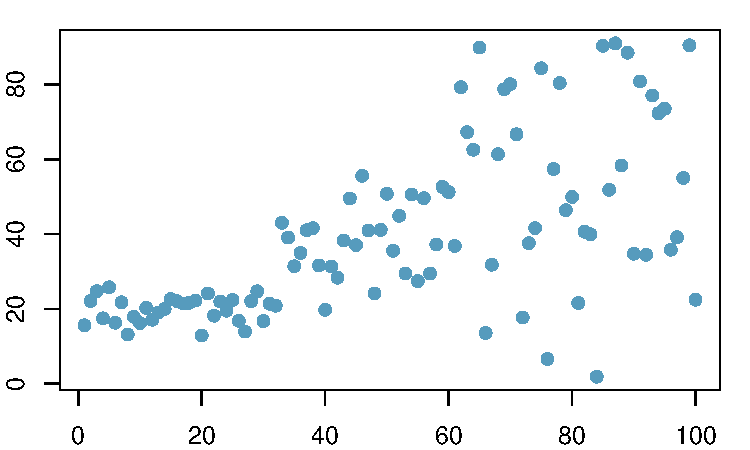
\includegraphics[width=0.4\textwidth]{figures/nonconstant_var}
\end{center}
\item Derive the formula for $b_0$ given the fact that the linear model is $\hat{y} = b_0 + b_1 \times x$ and that the least squares line goes through ($\bar{x}, \bar{y}$).
\item One study on male college students found their average height to be 70 inches with a standard deviation of 2 inches. Their average weight was 140 pounds, with a standard deviation of 25 pounds. The correlation between their height and weight was 0.60. Assuming that the two variables are linearly associated, write the linear model for predicting weight from height.
\item Is a male who is 72 inches tall and who weighs 115 pounds on the line, below the line, or above the line?
\item Describe what is an indicator variable, and what levels 0 and 1 mean for such variables.
\item The model below predicts GPA based on an indicator variable (0: not premed, 1: premed). Interpret the intercept and slope estimates in context of the data.
\[ \widehat{gpa} = 3.57 - 0.01 \times premed \]
\item If the correlation between two variables $y$ and $x$ is 0.6, what percent of the variability in $y$ does $x$ explain? 
\end{enumerate}
\end{itemize}
}}

%

\vspace{0.48cm}

%

\begin{enumerate}[resume]
\renewcommand\labelenumi{\textcolor{light}{\textbf{LO \theenumi.}}}

\item Define a leverage point as a point that lies away from the center of the data in the horizontal direction.

\item Define an influential point as a point that influences (changes) the slope of the regression line.
\begin{itemize}
\item[-] This is usually a leverage point that is away from the trajectory of the rest of the data.
\end{itemize}

\item Do not remove outliers from an analysis without good reason.

\item Be cautious about using a categorical explanatory variable when one of the levels has very few observations, as these may act as influential points.

\end{enumerate}

\gray{
{\it
\vspace{-0.55cm}
\begin{itemize}
\renewcommand{\labelitemi}{{\textcolor{dark}{$\ast$}}}
\item Reading: Section 8.3 of OpenIntro Statistics
\item Videos: To be posted 
\item Test yourself: Determine if each of the three unusual observations in the plot below would be considered just an outlier, a leverage point, or an influential point.
\begin{center}
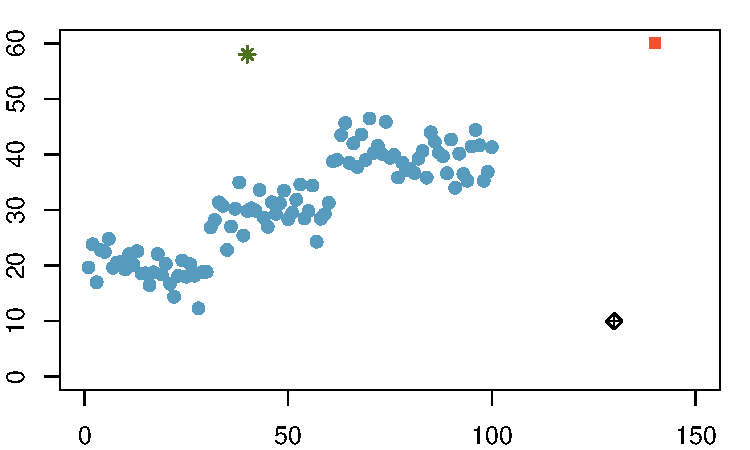
\includegraphics[width=0.5\textwidth]{figures/outliers}
\end{center}
\end{itemize}
}}

%

\vspace{0.48cm}

%

\begin{enumerate}[resume]
\renewcommand\labelenumi{\textcolor{light}{\textbf{LO \theenumi.}}}

\item Determine whether an explanatory variable is a significant predictor for the response variable using the $t$-test and the associated p-value in the regression output.

\item Set the null hypothesis testing for the significance of the predictor as $H_0: \beta_1 = 0$, and recognize that the standard software output yields the p-value for the two-sided alternative hypothesis.
\begin{itemize}
\item[-] Note that $\beta_1 = 0$ means the regression line is horizontal, hence suggesting that there is no relationship between the explanatory and the response variables.
\end{itemize}

\item Calculate the T score for the hypothesis test as 
\[ T_{df} = \frac{b_1 - \text{null value}}{SE_{b_1}} \]
with $df = n - 2$.
\begin{itemize}
\item[-] Note that the T score has $n - 2$ degrees of freedom since we lose one degree of freedom for each parameter we estimate, and in this case we estimate the intercept and the slope.
\end{itemize}

\item Note that a hypothesis test for the intercept is often irrelevant since it's usually out of the range of the data, and hence it is usually an extrapolation.

\item Calculate a confidence interval for the slope as
\[ b_1 \pm t^\star_{df} SE_{b_1}, \]
where $df = n - 2$ and $t^\star_{df}$ is the critical score associated with the given confidence level at the desired degrees of freedom.
\begin{itemize}
\item[-] Note that the standard error of the slope estimate $SE_{b_1}$ can be found on the regression output.
\end{itemize}

\end{enumerate}

\gray{
{\it
\vspace{-0.55cm}
\begin{itemize}
\renewcommand{\labelitemi}{{\textcolor{dark}{$\ast$}}}
\item Reading: Section 8.4 of OpenIntro Statistics
\item Videos: To be posted 
\item Test yourself: 
\begin{enumerate}
\item Given the regression output below for predicting $y$ from $x$ where $n = 100$, confirm the T score and the p-value, determine whether $x$ is a significant predictor of $y$, and interpret the p-value in context.
\begin{center}
\begin{tabular}{rrrrr}
  \hline
 & Estimate & Std. Error & t value & Pr($>$$|$t$|$) \\ 
  \hline
(Intercept) & 19.8581 & 6.1379 & 3.24 & 0.0017 \\ 
  x & 0.2557 & 0.1055 & 2.42 & 0.0172 \\ 
   \hline
\end{tabular}
\end{center}
\item Calculate a 95\% confidence interval for the slope given above.
\end{enumerate}
\end{itemize}
}}

\end{document}